\documentclass{prova}

\usepackage{amsmath}
\usepackage{amsfonts}

\setlength{\textheight}{25cm}

\DeclareMathOperator{\sen}{sen}
\DeclareMathOperator{\tg}{tg}
\newcommand{\ds}{\displaystyle}

\professor{Prof.\@ Adriano Barbosa}
\disciplina{C\'alculo Diferencial e Integral}
\avaliacao{P2}
\curso{F\'{\i}sica}
\data{06/06/2022}

\begin{document}
	\cabecalho{5}  % o numero 5 indica a qnt de quadros na tabela de nota

    \textbf{Todas as respostas devem ser justificadas.}

    \begin{questionario}
        \q{Calcule o limite $\displaystyle\lim_{x\rightarrow 0^{+}}
           x^{\sqrt{x}}$.}

        \q{Um tanque cil\'{\i}ndrico com raio 3m est\'a enchendo com \'agua a uma taxa
           de 2m$^3$/min. Qu\~ao r\'apido a altura da \'agua est\'a aumentando?}

        \q{Explique o efeito de cada linha abaixo no gr\'afico de $f$ e esboce o
           gr\'afico da fun\c{c}\~ao tal que:}

            $f(0)=0, f'(-1)=f'(3)=0$ \\
            $\displaystyle\lim_{x\rightarrow -\infty}f(x) =\lim_{x\rightarrow
            +\infty} f(x) =0$ \\
            $f'(x)<0$ em $(-\infty,-1)$ e $(3,+\infty)$ \\
            $f'(x)>0$ em $(-1,3)$ \\
            $f''(x)>0$ em $(-2,0)$ e $(5,+\infty)$ \\
            $f''(x)<0$ em $(-\infty,-2)$ e $(0,5)$

        \q{Calcule a \'area entre as curvas $y=x^2-\frac{8}{3}x$ e
           $y=\frac{1}{3}x$.}
            \begin{figure}[h]
                \centering
                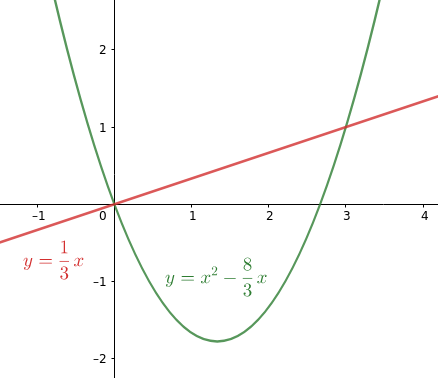
\includegraphics[width=0.4\textwidth]{fig1.png}
            \end{figure}

        \q{Calcule o volume da regi\~ao delimitada por $y=2x$, $y=x^2$
           rotacionada ao redor do eixo $x$.}
    \end{questionario}
\end{document}
